\documentclass[../main.tex]{subfile}
\graphicspath{{\subfix{../images}}}
\begin{document}

人们只要撇图片一眼就可以立即知道什么物体在图片中、它们在哪里以及它们是如何交互的。人类的视觉系统是快速且准确的,这允许我们在不那么小心的情况下去进行例如开车的复杂任务。快速且准确的检测算法将会允许计算机在没有专门传感器的情况下驾驶汽车、使得辅助设备可以传输实时场景信息给人类用户、并释放通用响应机器人系统的潜力。

目前的检测系统通过复用分类器来进行检测。为了检测一个物体,这些系统为该对象使用一个分类器,并在测试图像中的不同位置和不同尺度对其进行评估。可变部件模型(DPM)等系统使用滑动窗口方法,其中分类器在整个图像上的均匀间隔的位置运行\cite{dpm}。

最近的方法如R-CNN通过区域候选的方法首先在图像中生成潜在的边界框,然后在这些候选框上运行分类器。分类后,通过后处理来微调边界框、消除重复检测,并根据场景中的其他对象对框重新评分\cite{rcnn}。因为必须单独训练复杂管道中的每个单独组件,所以这些管道速度缓慢且难以优化。

我们将目标检测重新定义为一个单一的回归问题,直接从图像像素到边界框坐标和类别概率。使用我们的系统,只需查看图像一次 (YOLO) 即可预测存在哪些对象以及它们在哪里。

\begin{figure}[htb]
    \centering
    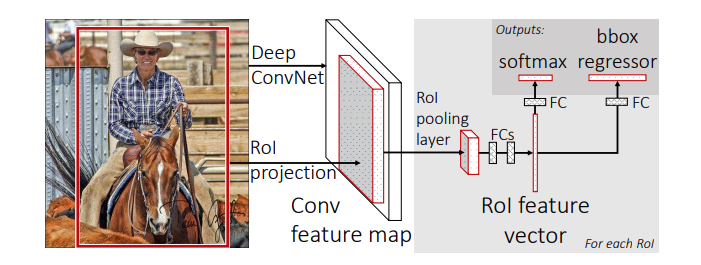
\includegraphics[width=\textwidth]{fig1.png}
    \caption{\textbf{YOLO检测系统}使用 YOLO 处理图像简单明了。我们的系统(1)将输入图像的大小调整为$ 448 \times 448$,(2)在图像上运行单个卷积网络,以及(3)通过模型的置信度对结果检测进行阈值处理。}
    \label{fig:fig1}
\end{figure}

YOLO 非常简单:见图\ref{fig:fig1}。单个卷积网络同时预测多个边界框和这些框的类别概率。YOLO在完整图像上训练并直接优化检测性能。与传统的对象检测方法相比,这种统一模型有多个优点。

首先,YOLO非常快。由于我们将检测视为回归问题,因此我们不需要复杂的管道。我们只是在测试时在新图像上运行我们的神经网络来预测检测。在Titan X GPU上且没有批处理的情况下,我们的基础网络达到了每秒45帧的运行速度,快速版本达到了超过150 fps的运行速度。这意味着我们可以以不到25毫秒的延迟实时处理流视频。此外,YOLO的平均精度是其他实时系统平均精度的两倍以上。有关我们系统在网络摄像头上实时运行的演示,请参阅我们的项目网页:\href{http://pjreddie.com/yolo/}{http://pjreddie.com/yolo/}。

其次,YOLO在进行预测时会对图像进行全局推理。与基于滑动窗口和区域候选的技术不同,YOLO在训练和测试期间看到整个图像,因此它隐式编码了关于类及其外观的上下文信息。Fast R-CNN是一种顶级检测方法\cite{fastrcnn},由于无法看到更大的上下文,因此会将图像中的背景块误认为是物体。与Fast R-CNN相比,YOLO的背景误报数量不到一半。

第三,YOLO学习对象的可泛化表示。在对自然图像进行训练并在艺术品上进行测试时,YOLO的性能大大优于DPM和R-CNN等顶级检测方法。由于YOLO具有高度泛化性,因此在应用于新领域或意外输入时不太可能崩溃。

YOLO在准确性方面仍然落后于最先进的检测系统。虽然它可以快速识别图像中的物体,但它很难精确定位一些物体,尤其是小物体。我们在实验中进一步研究了这些权衡。

我们所有的训练和测试代码都是开源的。还可以下载各种预训练模型。

\end{document}